%%%%%%%%%%%%%%%%%%%%%%%%%%%%%%%%%%%%%%%%%%%
%%%%%%  STYLE 06
%%%%%%%%%%%%%%%%%%%%%%%%%%%%%%%%%%%%%%%%%%%

\cxset{style06/.style={
 name={Chapter},
 numbering=arabic,
 number font-size=\Huge,
 number font-family=\calligra,
 number font-weight=\calligra,
 number color=\color{black!90},
 number before=\kern-2.5pt,
 number dot=,
 number after=,
 number position=rightname,
 chapter font-family=\rmfamily,
 chapter font-weight=\calligra,
 chapter font-size=\LARGE\calligra,
 chapter before={\vspace*{20pt}\par\hfill},
 chapter after={\hfill\hfill\par},
 chapter color={black!90},
 title beforeskip={\vspace*{50pt}},
 title afterskip={\vspace{3.5pt}\par},
 title before={\hfill},
 title after={\hfill\hfill},
 title font-family=\rmfamily,
 title font-color=\color{black!90},
 title font-weight=\normalfont,
 title font-size=\LARGE,
 title spaceout=soul,
}}

\cxset{style06}

\chapter{INTRODUCTION TO STYLE SIX}
\renewcommand{\DefaultLhang}{0.1}
\renewcommand{\LettrineFontHook}{\calligra}
\setlength{\DefaultFindent}{9.5pt}
\setlength{\DefaultNindent}{0pt}

\lettrine{\textcolor{orange}{T}}{}he calligraphic font for this design make it stand out, although you may need to experiment to get the right font (I have used calligra). I am sure the specification can be optimized a bit, however so far it works. I also opted to space out the title. I had to experiment a bit to get the Lettrine settings.
\medskip
\begin{figure}[ht]
\centering
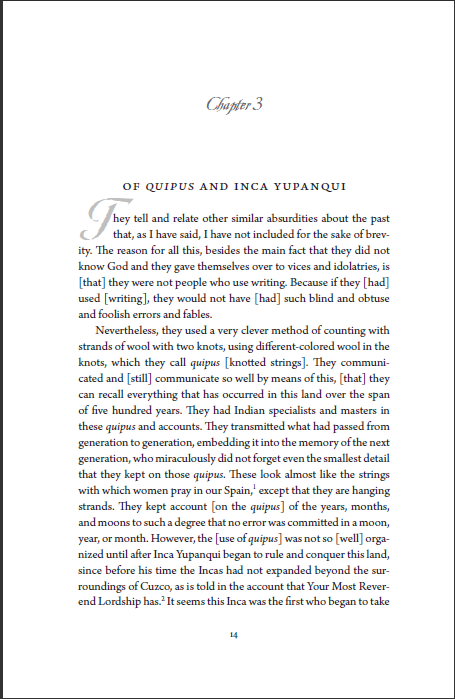
\includegraphics[width=0.6\textwidth]{./chapters/chapter06}
\end{figure}

The number has been kerned using:

\begin{lstlisting}
 number before=\kern-4.5pt,
\end{lstlisting}

This template has a lot of potential and I will come back to it and add more key hooks for lettrine settings per letter and font management. They can also come alive with a gold color.

